\documentclass[11pt]{article}
\title{\textbf{Meccano hexagons}}
\author{https://github.com/heptagons/meccano/hexa}
\date{}

\usepackage{amsmath}
\usepackage{listings}
\usepackage{xcolor}
\definecolor{gray}{RGB}{245,245,245}

\lstset{
	backgroundcolor=\color{gray},
	frame=single,
	language=c,
	numbers=left,
	stepnumber=1
}


\usepackage[margin=0.75in]{geometry}

\usepackage{tikz}
\usetikzlibrary{math}

\usepackage{graphicx}

\begin{document}

\maketitle

\section{Meccano hexagons}

A meccano hexagon can be formed easily attaching equilateral
triangles as small as one unit side. Also joining six unit bars and using
double bars twice a rigid hexagon side $1$ is obtained as shown in figure \ref{fig:1}.
Next we will find a way to make more interesting hexagons with diagonals with lengths not exact
multiples of hexagon side.

\begin{figure}[htpb]
\centering
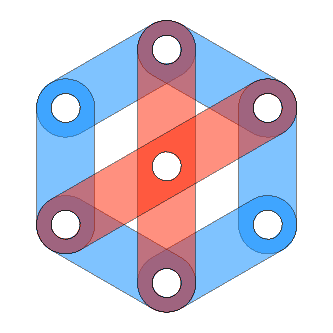
\includegraphics[scale=0.5]{figs/hexagon-1}
\caption{Rigid hexagon. Six blue bars form the perimeter with two double
diagonals in red.}
\label{fig:1}
\end{figure}


\begin{figure}[htpb]
\centering
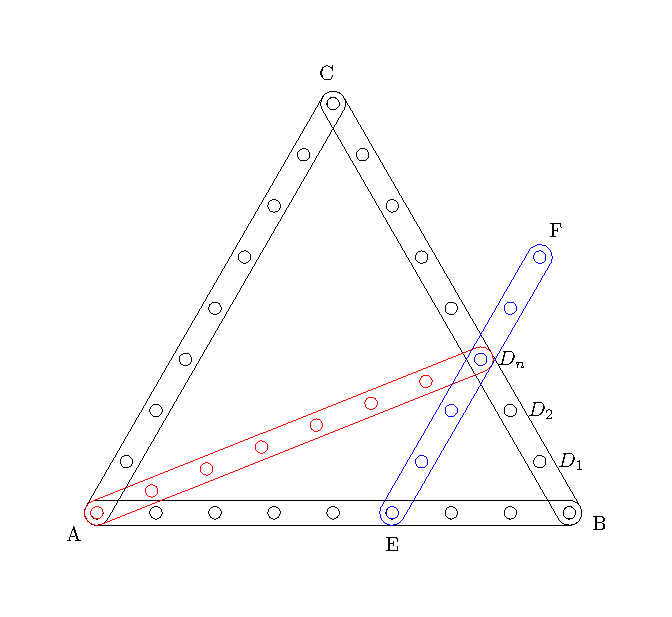
\includegraphics[scale=0.8]{hexagon_angle}
\caption{Regular hexagon internal angle plan. Consider an equilateral triangle $ABC$.
Try to connect a new rod from point $A$ to several points $D$ located 
over the bar $\overline{BC}$
in such a way length $\overline{AD}$ is an integer.
If so, connect a new rod $\overline{EF}$ where $\overline{EB} = \overline{BC}$ and $\overline{EF} = \overline{AE}$. Angle $AEF$ is the internal regular hexagon angle ($120^\circ{}$).}
\label{fig:plan}
\end{figure}

\subsection{Independent diagonals}

Figure \ref{fig:plan} shows a plan to find independent diagonals that form the regular hexagon internal angles.
From the figure the angle at $B$ is fixed to $60^\circ{}$, since $ABC$ is a
(rigid) equilateral triangle.
Let $a$ and $b$ two integers such as $b <= a/2$.

We are looking for a third integer $d$ to be the independent diagonal:
\begin{align*}
a &= \overline{AB}\\
b &= \overline{BD} <= \frac{a}{2}\\
d &= \overline{AD}\\
e &= \overline{AE}
\end{align*}

Acording to cosines law, the diagonal value is calculated as follows:
\begin{align*}
d^2 &= a^2 + b^2 - 2ab\cos{\frac{\pi}{3}}\\
    &= a^2 + b^2 - ab\\
    &= (a-b)^2 + ab\\
    &= e^2 + ab
\end{align*}

Then, we need a program to iterate over integers $a$, then over integers $b$ to inspect whether $d$ value is as an integer too.

\subsection{Search of integer diagonals}

Next golang program find first cases.
We iterate from $a=1$ to a given maximum (line 2).
Then we iterate from $b=0$ to $b <= a/2$ (line 3).
In order to reject repetitions by scaling we check for greatest commond divisor
of $a$ and $b$ to be $1$ (line 4).
Then we calculate the diagonal using the plan's formula (line 5) and accept
only the case when the diagonal is a square number (line 8). 

\begin{lstlisting}
func triangle_diagonals(max int) {
  for a := 1; a < max; a++ {
    for b := 1; b <= a/2; b++ {
      if gcd(a, b) == 1 {
        diag := (a-b)*(a-b) + a*b
        cd := math.Sqrt(float64(diag))
        d := int(cd)
        if cd == float64(d) {
          num := float64(diag + a*a - b*b)
          den := 2.0 * cd * float64(a)
          angle := 180*math.Acos(num/den)/math.Pi
          fmt.Printf("a=%3d b=%3d d=%3d angle=%8.4f\n", a, b, d, angle)
        }
      }
    }
  }
}
func gcd(a, b int) int { // greatest common divisor
  if b == 0 {
    return a
  }
  return gcd(b, a % b)
}
\end{lstlisting}

\subsection{Integral diagonals results}
The program found $13$ cases with integral diagonals for hexagons side $<= 100$.
Each result includes lenghts $a$, $b$, $d$ and the angle $DAE$ (see figure \ref{fig:plan}).

\begin{lstlisting}
a=  8 b=  3 d=  7 angle= 21.7868
a= 15 b=  7 d= 13 angle= 27.7958
a= 21 b=  5 d= 19 angle= 13.1736
a= 35 b= 11 d= 31 angle= 17.8966
a= 40 b=  7 d= 37 angle=  9.4300
a= 48 b= 13 d= 43 angle= 15.1782
a= 55 b= 16 d= 49 angle= 16.4264
a= 65 b=  9 d= 61 angle=  7.3410
a= 77 b= 32 d= 67 angle= 24.4327
a= 80 b= 17 d= 73 angle= 11.6351
a= 91 b= 40 d= 79 angle= 26.0078
a= 96 b= 11 d= 91 angle=  6.0090
a= 99 b= 19 d= 91 angle= 10.4174
\end{lstlisting}

\subsection{Examples}

\begin{figure}
\centering
\scalebox{0.8}{
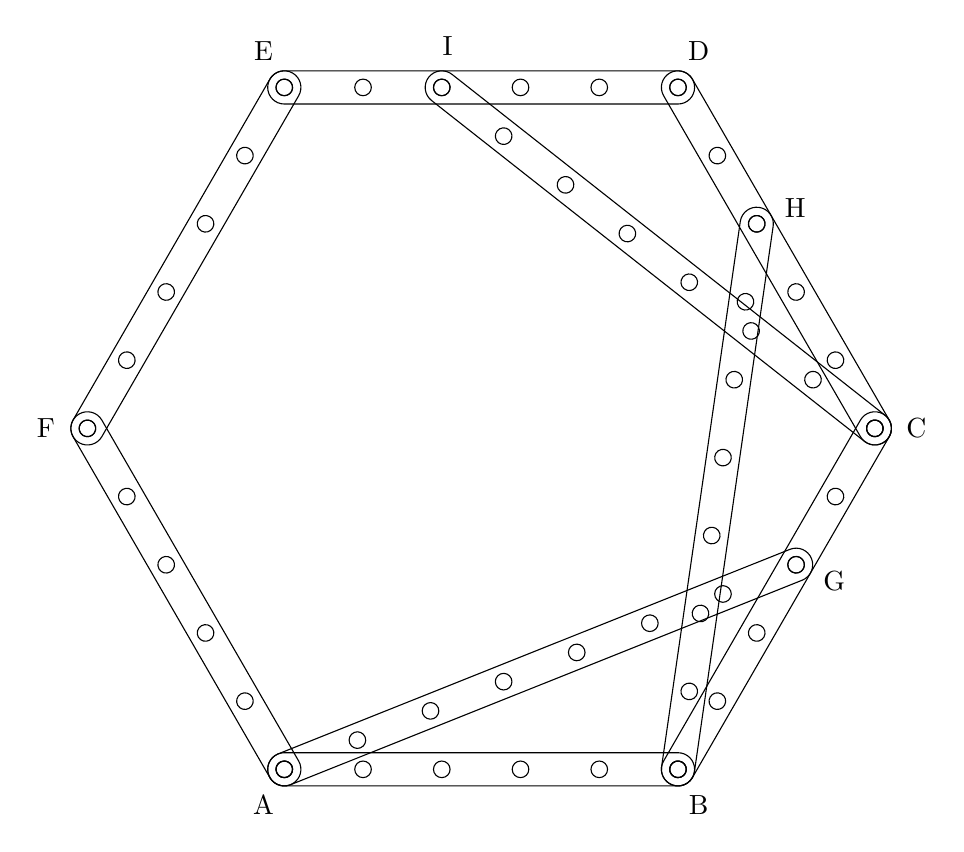
\begin{tikzpicture}

\begin{scope} %AB
 \def\s{5}
 \def\t{7}
 \def\r{21.7868}
 \draw (0,6pt) -- ++(\s,0) arc(+90:-90:6pt) -- ++(-\s,0) arc(270:90:6pt);
 \foreach \x in {0,1,...,\s} 
 \draw (\x,0) circle (3pt);
 \path (0,0) ++(240:15pt) node{A};

 \begin{scope}[rotate=\r] %AG
  \draw (0,6pt) -- ++(\t,0) arc(+90:-90:6pt) -- ++(-\t,0) arc(270:90:6pt);
  \foreach \x in {0,1,...,\t} 
  \draw (\x,0) circle (3pt);
  \path (\t,0) ++(-45:15pt) node{G};
 \end{scope}

 \begin{scope}[shift={(\s,0)},rotate=60] %BC
  \draw (0,6pt) -- ++(\s,0) arc(+90:-90:6pt) -- ++(-\s,0) arc(270:90:6pt);
  \foreach \x in {0,1,...,\s} 
  \draw (\x,0) circle (3pt);
  \path (0,0) ++(240:15pt) node{B};

  \begin{scope}[rotate=\r] %BH
   \draw (0,6pt) -- ++(\t,0) arc(+90:-90:6pt) -- ++(-\t,0) arc(270:90:6pt);
   \foreach \x in {0,1,...,\t} 
   \draw (\x,0) circle (3pt);
   \path (\t,0) ++(-60:15pt) node{H};
  \end{scope}

  \begin{scope}[shift={(\s,0)},rotate=60] %CD
   \draw (0,6pt) -- ++(\s,0) arc(+90:-90:6pt) -- ++(-\s,0) arc(270:90:6pt);
   \foreach \x in {0,1,...,\s} 
   \draw (\x,0) circle (3pt);
   \path (0,0) ++(240:15pt) node{C};
   
   \begin{scope}[rotate=\r] %CI
    \draw (0,6pt) -- ++(\t,0) arc(+90:-90:6pt) -- ++(-\t,0) arc(270:90:6pt);
    \foreach \x in {0,1,...,\t} 
    \draw (\x,0) circle (3pt);
    \path (\t,0) ++(-60:15pt) node{I};
   \end{scope}

   \begin{scope}[shift={(\s,0)},rotate=60] %DE
    \draw (0,6pt) -- ++(\s,0) arc(+90:-90:6pt) -- ++(-\s,0) arc(270:90:6pt);
    \foreach \x in {0,1,...,\s} 
    \draw (\x,0) circle (3pt);
    \path (0,0) ++(240:15pt) node{D};
    
    \begin{scope}[shift={(\s,0)},rotate=60]
     \draw (0,6pt) -- ++(\s,0) arc(+90:-90:6pt) -- ++(-\s,0) arc(270:90:6pt);
     \foreach \x in {0,1,...,\s} 
     \draw (\x,0) circle (3pt);
     \path (0,0) ++(240:15pt) node{E};

     \begin{scope}[shift={(\s,0)},rotate=60] %EF
      \draw (0,6pt) -- ++(\s,0) arc(+90:-90:6pt) -- ++(-\s,0) arc(270:90:6pt);
      \foreach \x in {0,1,...,\s} 
      \draw (\x,0) circle (3pt);
      \path (0,0) ++(240:15pt) node{F};
     \end{scope}

    \end{scope}
    
   \end{scope}   
   
  \end{scope}

 \end{scope}

\end{scope}

\end{tikzpicture}
}
\caption{Hexagon sides $5$, diagonals $7$.}
\label{fig:5-7}
\end{figure}


\begin{figure}
\centering
\scalebox{1}{
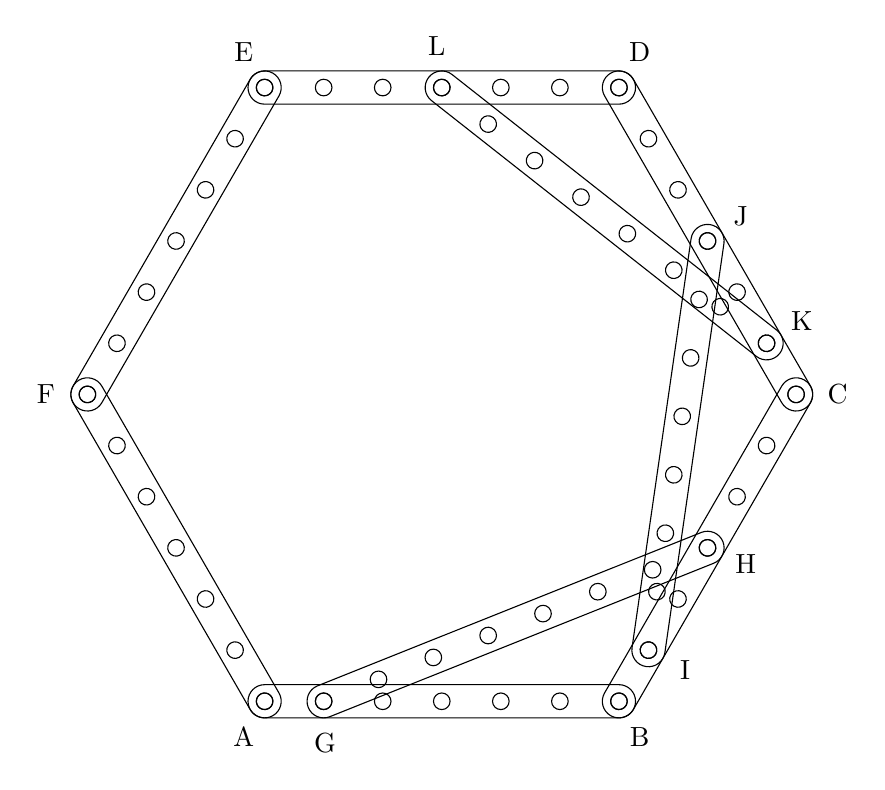
\begin{tikzpicture}

\def\p{3pt} \def\u{0.75} \def\s{6} \def\t{7} \def\r{21.7868}
\begin{scope} %AB
 \draw (0,2*\p) -- ++(\s*\u,0) arc(+90:-90:2*\p) -- ++(-\s*\u,0) arc(270:90:2*\p);
 \foreach \x in {0,1,...,\s} \draw (\x*\u,0) circle (\p);
 \path (0,0) ++(240:5*\p) node{A};

 \begin{scope}[shift={(1*\u,0)},rotate=\r] %GH
  \draw (0,2*\p) -- ++(\t*\u,0) arc(+90:-90:2*\p) -- ++(-\t*\u,0) arc(270:90:2*\p);
  \foreach \x in {0,1,...,\t} \draw (\x*\u,0) circle (\p);
  \path (0,0) ++(-110:5*\p) node{G};
  \path (\t*\u,0) ++(-45:5*\p) node{H};
 \end{scope}

 \begin{scope}[shift={(\s*\u,0)},rotate=60] %BC
  \draw (0,2*\p) -- ++(\s*\u,0) arc(+90:-90:2*\p) -- ++(-\s*\u,0) arc(270:90:2*\p);
  \foreach \x in {0,1,...,\s} \draw (\x*\u,0) circle (\p);
  \path (0,0) ++(240:5*\p) node{B};

  \begin{scope}[shift={(1*\u,0)},rotate=\r] %IJ
   \draw (0,2*\p) -- ++(\t*\u,0) arc(+90:-90:2*\p) -- ++(-\t*\u,0) arc(270:90:2*\p);
   \foreach \x in {0,1,...,\t} \draw (\x*\u,0) circle (\p);
   \path (0,0) ++(-110:5*\p) node{I};
   \path (\t*\u,0) ++(-45:5*\p) node{J};
  \end{scope}

  \begin{scope}[shift={(\s*\u,0)},rotate=60] %CD
   \draw (0,2*\p) -- ++(\s*\u,0) arc(+90:-90:2*\p) -- ++(-\s*\u,0) arc(270:90:2*\p);
   \foreach \x in {0,1,...,\s} \draw (\x*\u,0) circle (\p);
   \path (0,0) ++(240:5*\p) node{C};
   
   \begin{scope}[shift={(1*\u,0)},rotate=\r] %KL
    \draw (0,6pt) -- ++(\t*\u,0) arc(+90:-90:6pt) -- ++(-\t*\u,0) arc(270:90:6pt);
    \foreach \x in {0,1,...,\t} \draw (\x*\u,0) circle (\p);
    \path (0,0) ++(-110:5*\p) node{K};
    \path (\t*\u,0) ++(-45:5*\p) node{L};
   \end{scope}

   \begin{scope}[shift={(\s*\u,0)},rotate=60] %DE
    \draw (0,2*\p) -- ++(\s*\u,0) arc(+90:-90:2*\p) -- ++(-\s*\u,0) arc(270:90:2*\p);
    \foreach \x in {0,1,...,\s} \draw (\x*\u,0) circle (\p);
    \path (0,0) ++(240:5*\p) node{D};
    
    \begin{scope}[shift={(\s*\u,0)},rotate=60]
     \draw (0,2*\p) -- ++(\s*\u,0) arc(+90:-90:2*\p) -- ++(-\s*\u,0) arc(270:90:2*\p);
     \foreach \x in {0,1,...,\s} \draw (\x*\u,0) circle (\p);
     \path (0,0) ++(240:5*\p) node{E};

     \begin{scope}[shift={(\s*\u,0)},rotate=60] %EF
      \draw (0,2*\p) -- ++(\s*\u,0) arc(+90:-90:2*\p) -- ++(-\s*\u,0) arc(270:90:2*\p);
      \foreach \x in {0,1,...,\s} \draw (\x*\u,0) circle (\p);
      \path (0,0) ++(240:5*\p) node{F};
     \end{scope}

    \end{scope}
    
   \end{scope}   
   
  \end{scope}

 \end{scope}

\end{scope}

\end{tikzpicture}
}
\caption{Hexagon sides $5+1=6$, diagonals $7$. }
\label{fig:6-7}
\end{figure}



\begin{figure}
\centering
\scalebox{0.7}{
\begin{tikzpicture}

\begin{scope} %AB
 \def\p{3pt} \def\u{1.33} \def\s{7} \def\t{7} \def\r{21.7868}
 \draw (0,2*\p) -- ++(\s*\u,0) arc(+90:-90:2*\p) -- ++(-\s*\u,0) arc(270:90:2*\p);
 \foreach \x in {0,1,...,\s} \draw (\x*\u,0) circle (\p);
 \path (0,0) ++(240:5*\p) node{A};

 \begin{scope}[shift={(2*\u,0)},rotate=\r] %AG
  \draw (0,2*\p) -- ++(\t*\u,0) arc(+90:-90:2*\p) -- ++(-\t*\u,0) arc(270:90:2*\p);
  \foreach \x in {0,1,...,\t} \draw (\x*\u,0) circle (\p);
  \path (\t*\u,0) ++(-45:5*\p) node{G};
 \end{scope}

 \begin{scope}[shift={(\s*\u,0)},rotate=60] %BC
  \draw (0,2*\p) -- ++(\s*\u,0) arc(+90:-90:2*\p) -- ++(-\s*\u,0) arc(270:90:2*\p);
  \foreach \x in {0,1,...,\s} \draw (\x*\u,0) circle (\p);
  \path (0,0) ++(240:5*\p) node{B};

  \begin{scope}[shift={(2*\u,0)},rotate=\r] %BH
   \draw (0,2*\p) -- ++(\t*\u,0) arc(+90:-90:2*\p) -- ++(-\t*\u,0) arc(270:90:2*\p);
   \foreach \x in {0,1,...,\t} \draw (\x*\u,0) circle (\p);
   \path (\t*\u,0) ++(-60:5*\p) node{H};
  \end{scope}

  \begin{scope}[shift={(\s*\u,0)},rotate=60] %CD
   \draw (0,2*\p) -- ++(\s*\u,0) arc(+90:-90:2*\p) -- ++(-\s*\u,0) arc(270:90:2*\p);
   \foreach \x in {0,1,...,\s} \draw (\x*\u,0) circle (\p);
   \path (0,0) ++(240:5*\p) node{C};
   
   \begin{scope}[shift={(2*\u,0)},rotate=\r] %CI
    \draw (0,6pt) -- ++(\t*\u,0) arc(+90:-90:6pt) -- ++(-\t*\u,0) arc(270:90:6pt);
    \foreach \x in {0,1,...,\t} \draw (\x*\u,0) circle (\p);
    \path (\t*\u,0) ++(-60:5*\p) node{I};
   \end{scope}

   \begin{scope}[shift={(\s*\u,0)},rotate=60] %DE
    \draw (0,2*\p) -- ++(\s*\u,0) arc(+90:-90:2*\p) -- ++(-\s*\u,0) arc(270:90:2*\p);
    \foreach \x in {0,1,...,\s} \draw (\x*\u,0) circle (\p);
    \path (0,0) ++(240:5*\p) node{D};
    
    \begin{scope}[shift={(\s*\u,0)},rotate=60]
     \draw (0,2*\p) -- ++(\s*\u,0) arc(+90:-90:2*\p) -- ++(-\s*\u,0) arc(270:90:2*\p);
     \foreach \x in {0,1,...,\s} \draw (\x*\u,0) circle (\p);
     \path (0,0) ++(240:5*\p) node{E};

     \begin{scope}[shift={(\s*\u,0)},rotate=60] %EF
      \draw (0,2*\p) -- ++(\s*\u,0) arc(+90:-90:2*\p) -- ++(-\s*\u,0) arc(270:90:2*\p);
      \foreach \x in {0,1,...,\s} \draw (\x*\u,0) circle (\p);
      \path (0,0) ++(240:5*\p) node{F};
     \end{scope}

    \end{scope}
    
   \end{scope}   
   
  \end{scope}

 \end{scope}

\end{scope}

\end{tikzpicture}

}
\caption{Hexagon sides $5+2=7$, diagonals $7$.}
\label{fig:7-7}
\end{figure}




\begin{figure}
\centering
\scalebox{1}{
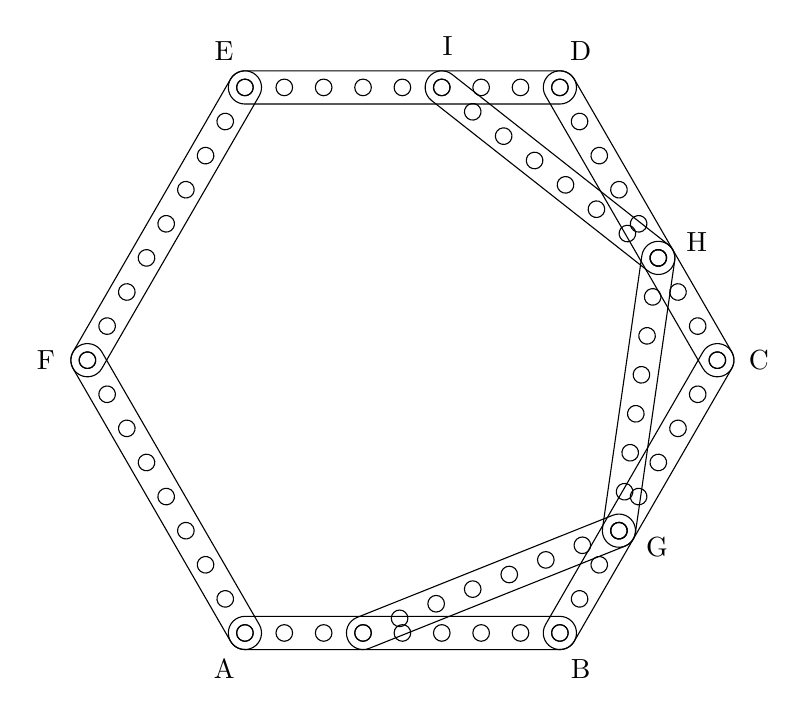
\begin{tikzpicture}

\begin{scope} %AB
 \def\p{3pt} \def\u{0.5} \def\s{8} \def\t{7} \def\r{21.7868}
 \draw (0,2*\p) -- ++(\s*\u,0) arc(+90:-90:2*\p) -- ++(-\s*\u,0) arc(270:90:2*\p);
 \foreach \x in {0,1,...,\s} \draw (\x*\u,0) circle (\p);
 \path (0,0) ++(240:5*\p) node{A};

 \begin{scope}[shift={(3*\u,0)},rotate=\r] %AG
  \draw (0,2*\p) -- ++(\t*\u,0) arc(+90:-90:2*\p) -- ++(-\t*\u,0) arc(270:90:2*\p);
  \foreach \x in {0,1,...,\t} \draw (\x*\u,0) circle (\p);
  \path (\t*\u,0) ++(-45:5*\p) node{G};
 \end{scope}

 \begin{scope}[shift={(\s*\u,0)},rotate=60] %BC
  \draw (0,2*\p) -- ++(\s*\u,0) arc(+90:-90:2*\p) -- ++(-\s*\u,0) arc(270:90:2*\p);
  \foreach \x in {0,1,...,\s} \draw (\x*\u,0) circle (\p);
  \path (0,0) ++(240:5*\p) node{B};

  \begin{scope}[shift={(3*\u,0)},rotate=\r] %BH
   \draw (0,2*\p) -- ++(\t*\u,0) arc(+90:-90:2*\p) -- ++(-\t*\u,0) arc(270:90:2*\p);
   \foreach \x in {0,1,...,\t} \draw (\x*\u,0) circle (\p);
   \path (\t*\u,0) ++(-60:5*\p) node{H};
  \end{scope}

  \begin{scope}[shift={(\s*\u,0)},rotate=60] %CD
   \draw (0,2*\p) -- ++(\s*\u,0) arc(+90:-90:2*\p) -- ++(-\s*\u,0) arc(270:90:2*\p);
   \foreach \x in {0,1,...,\s} \draw (\x*\u,0) circle (\p);
   \path (0,0) ++(240:5*\p) node{C};
   
   \begin{scope}[shift={(3*\u,0)},rotate=\r] %CI
    \draw (0,6pt) -- ++(\t*\u,0) arc(+90:-90:6pt) -- ++(-\t*\u,0) arc(270:90:6pt);
    \foreach \x in {0,1,...,\t} \draw (\x*\u,0) circle (\p);
    \path (\t*\u,0) ++(-60:5*\p) node{I};
   \end{scope}

   \begin{scope}[shift={(\s*\u,0)},rotate=60] %DE
    \draw (0,2*\p) -- ++(\s*\u,0) arc(+90:-90:2*\p) -- ++(-\s*\u,0) arc(270:90:2*\p);
    \foreach \x in {0,1,...,\s} \draw (\x*\u,0) circle (\p);
    \path (0,0) ++(240:5*\p) node{D};
    
    \begin{scope}[shift={(\s*\u,0)},rotate=60]
     \draw (0,2*\p) -- ++(\s*\u,0) arc(+90:-90:2*\p) -- ++(-\s*\u,0) arc(270:90:2*\p);
     \foreach \x in {0,1,...,\s} \draw (\x*\u,0) circle (\p);
     \path (0,0) ++(240:5*\p) node{E};

     \begin{scope}[shift={(\s*\u,0)},rotate=60] %EF
      \draw (0,2*\p) -- ++(\s*\u,0) arc(+90:-90:2*\p) -- ++(-\s*\u,0) arc(270:90:2*\p);
      \foreach \x in {0,1,...,\s} \draw (\x*\u,0) circle (\p);
      \path (0,0) ++(240:5*\p) node{F};
     \end{scope}

    \end{scope}
    
   \end{scope}   
   
  \end{scope}

 \end{scope}

\end{scope}

\end{tikzpicture}
}
\caption{Hexagon sides $5+3=8$, diagonals $7$. }
\label{fig:8-7}
\end{figure}


\begin{figure}
\centering
\scalebox{1}{
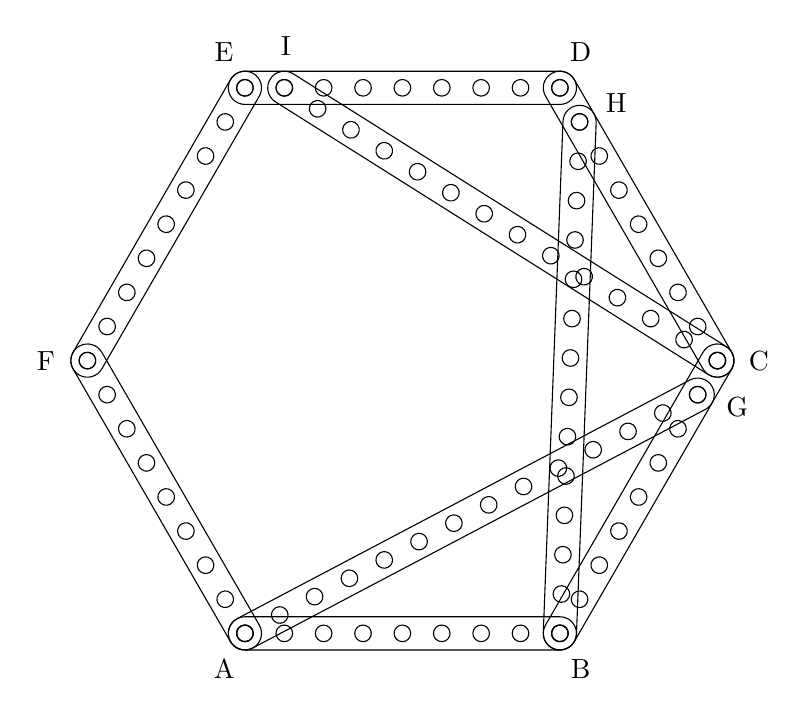
\begin{tikzpicture}

\def\p{3pt} \def\u{0.5} \def\s{8} \def\t{13} \def\r{27.7958}
\begin{scope} %AB
 \draw (0,2*\p) -- ++(\s*\u,0) arc(+90:-90:2*\p) -- ++(-\s*\u,0) arc(270:90:2*\p);
 \foreach \x in {0,1,...,\s} \draw (\x*\u,0) circle (\p);
 \path (0,0) ++(240:5*\p) node{A};

 \begin{scope}[rotate=\r] %AG
  \draw (0,2*\p) -- ++(\t*\u,0) arc(+90:-90:2*\p) -- ++(-\t*\u,0) arc(270:90:2*\p);
  \foreach \x in {0,1,...,\t} \draw (\x*\u,0) circle (\p);
  \path (\t*\u,0) ++(-45:5*\p) node{G};
 \end{scope}

 \begin{scope}[shift={(\s*\u,0)},rotate=60] %BC
  \draw (0,2*\p) -- ++(\s*\u,0) arc(+90:-90:2*\p) -- ++(-\s*\u,0) arc(270:90:2*\p);
  \foreach \x in {0,1,...,\s} \draw (\x*\u,0) circle (\p);
  \path (0,0) ++(240:5*\p) node{B};

  \begin{scope}[rotate=\r] %BH
   \draw (0,2*\p) -- ++(\t*\u,0) arc(+90:-90:2*\p) -- ++(-\t*\u,0) arc(270:90:2*\p);
   \foreach \x in {0,1,...,\t} \draw (\x*\u,0) circle (\p);
   \path (\t*\u,0) ++(-60:5*\p) node{H};
  \end{scope}

  \begin{scope}[shift={(\s*\u,0)},rotate=60] %CD
   \draw (0,2*\p) -- ++(\s*\u,0) arc(+90:-90:2*\p) -- ++(-\s*\u,0) arc(270:90:2*\p);
   \foreach \x in {0,1,...,\s} \draw (\x*\u,0) circle (\p);
   \path (0,0) ++(240:5*\p) node{C};
   
   \begin{scope}[rotate=\r] %CI
    \draw (0,6pt) -- ++(\t*\u,0) arc(+90:-90:6pt) -- ++(-\t*\u,0) arc(270:90:6pt);
    \foreach \x in {0,1,...,\t} \draw (\x*\u,0) circle (\p);
    \path (\t*\u,0) ++(-60:5*\p) node{I};
   \end{scope}

   \begin{scope}[shift={(\s*\u,0)},rotate=60] %DE
    \draw (0,2*\p) -- ++(\s*\u,0) arc(+90:-90:2*\p) -- ++(-\s*\u,0) arc(270:90:2*\p);
    \foreach \x in {0,1,...,\s} \draw (\x*\u,0) circle (\p);
    \path (0,0) ++(240:5*\p) node{D};
    
    \begin{scope}[shift={(\s*\u,0)},rotate=60]
     \draw (0,2*\p) -- ++(\s*\u,0) arc(+90:-90:2*\p) -- ++(-\s*\u,0) arc(270:90:2*\p);
     \foreach \x in {0,1,...,\s} \draw (\x*\u,0) circle (\p);
     \path (0,0) ++(240:5*\p) node{E};

     \begin{scope}[shift={(\s*\u,0)},rotate=60] %EF
      \draw (0,2*\p) -- ++(\s*\u,0) arc(+90:-90:2*\p) -- ++(-\s*\u,0) arc(270:90:2*\p);
      \foreach \x in {0,1,...,\s} \draw (\x*\u,0) circle (\p);
      \path (0,0) ++(240:5*\p) node{F};
     \end{scope}

    \end{scope}
    
   \end{scope}   
   
  \end{scope}

 \end{scope}

\end{scope}

\end{tikzpicture}
}
\caption{Hexagon sides $8$, diagonals $13$.}
\label{fig:8-13}
\end{figure}





\end{document}
